\chapter{Estudo de caso ? titulo ?}
\label{cap:estudodecaso}

Após os conceitos de alta disponibilidade e de virtualização terem sido compreendidos, pode-se iniciar a análise da estrutura atual da empresa.
Essa empresa, que fornece serviços de hospedagens, será o foco desse trabalho, sabendo que ela atualmente possui redundância de refrigeração 
e energia. Assim, essas redundâncias tem como objetivo prover um ambiente físico estável e confiável.

Para ser possível propor uma solução de alta diponibilidade é necessário conhecer o cenário atual da empresa, além de selecionar os serviços
mais críticos para a empresa. Então, nas próximas seções serão detalhados: o ambiente físico, com a estrutura e configuração dos servidores 
(Seção \ref{section:estfis}); a estrutura lógica, com a relação de servidores físicos e virtuais (Seção \ref{section:estlog}); todos os 
serviços fornecidos pela empresa (Seção \ref{section:serv}); e por fim a seleção dos serviços críticos (Seção \ref{section:servcrit}).

\section{Estrutura física}
\label{section:estfis}

A estrutura atual da empresa é composta por quatorze servidores físicos montados em um \textit{rack}. A configuração de \textit{hardware} desses 
servidores esta listado na Tabela \ref{tab:servfisicos}, que possui os campos nome do servidor, modelo e quantidade de processadores, quantidade
e tipo de memória, número de discos e a capacidade unitária, e o modelo e marca do servidor.

\begin{table}
\caption {Configuração dos servidores físicos}
\label{tab:servfisicos}
\begin{center}
\begin{tabular}{|l|p{3.8cm}|l|p{3cm}|l|}\hline
Servidor & Processador & Memória & Disco & Marca / modelo\\\hline
bello & Intel Core 2 Duo CPU E6750 2.66GHz & 2GB DDR2 & 5,5TB SATA & \\\hline
brina & 2 x Intel Xeon CPU E5410 2.33GHz & 24GB DDR2 & 6 x 300GB SAS & Dell PowerEdge 2950\\\hline
cacti & 2 x Intel Xeon CPU E5310 1.60GHz & 12GB DDR2 & 2 x 73GB SAS & Dell PowerEdge 2950\\\hline
dati & 2 x Intel Xeon CPU 3.20GHz & 4GB DDR2 & 2 x 146GB SCSI & Dell PowerEdge 1850\\\hline
fulmine & 1 x Intel Xeon CPU E5-2650 2.00GHz & 32GB DDR3 & 6 x 2TB SATA & IBM System x3650 M4\\\hline
monit & Intel Core 2 Quad CPU Q9550 2.83GHz & 4GB DDR2 & 120GB SSD & \\\hline
nino & Intel Core 2 Duo CPU E4500 2.20GHz & 4GB DDR2 & 500GB SATA & \\\hline
piova & 2 x Intel Xeon CPU E5530 2.40GHz & 32GB DDR3 & 4 x 500G SATA & Dell PowerEdge R410\\\hline
raggio & 2 x  Intel Xeon CPU E5630 2.53GHz & 32GB DDR3 & 4 x 300GB SAS & HP ProLiant DL360 G7\\\hline
sfrunhon & Intel Xeon CPU X3330 2.66GHz & 8GB DDR2 & 750GB SATA & \\\hline
tempesta & 2 x Intel Xeon CPU E5-2620 2.00GHz & 32GB DDR3 & 5 x 1TB SATA & Dell PowerEdge R620\\\hline
tuono & 2 x Intel Xeon CPU E5649 2.53GHz & 32GB DDR3 & 6 x 300GB SAS 2 x 146GB SAS & HP ProLiant DL380 G7\\\hline
venti & Intel Xeon CPU E3-1220 3.10GHz & 16GB DDR3 & 2 x 3TB SATA & Dell PowerEdge R210 II\\\hline
vigilante & Intel Pentium Dual CPU E2180 2.00GHz & 4GB DDR2 & 2,5TB SATA & \\\hline
\end{tabular}
\end{center}
\end{table}

%feito depois enviado para professor
Os servidores utilizados para virtualização possuem redundância de \textit{hardware}, com fonte de alimentação, discos configurados com \ac{RAID}, 
...

O diagrama (Figura \ref{fig:servfisicos}) demonstra a estrutura física....
%feito depois enviado para professor
Para cada servidor de virtualização dois cabos de rede são ligados a um \textit{switch} \textit{gigabit}, com isso possibilitando a configuração 
de \texit{link aggregation}, dobrando assim a capacidade de tráfego de dados...

\begin{figure}[servfisicos]
 \centering
 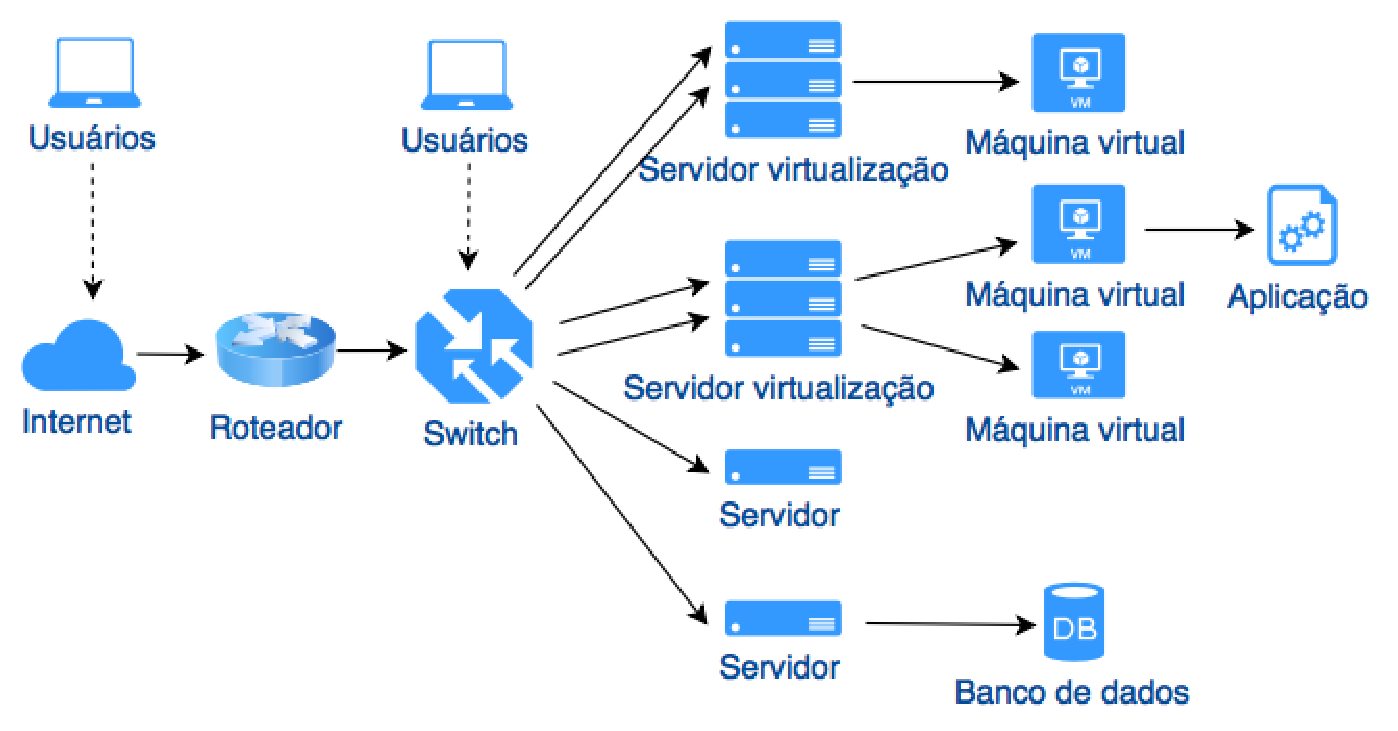
\includegraphics[width=180px]{img/servfisicos.eps}
 \caption{Estrutura física.}
 \label{fig:servfisicos}
\end{figure}

\section{Estrutura lógica}
\label{section:estlog}

Atualmente sete servidores são utilizados para virtualização, e os outros sete possuem serviços rodando diretamente. O primeiro servidor 
de virtualização (brina ? Como citar nome ?), que esta na Figura \ref{fig:servlog_1}, possui seis máquinas virtuais.
O segundo...

-diagramas máquinas de virtualização

%feito depois enviado para professor
Todos os servidores de virtualização possuem o sistema operacional \textit{Ubuntu} versão 14.04 LTS, para virtualização utilizam o hipervisor 
\ac{kvm} e \textit{qemu} para compor o ambiente de virtualização...

-graficos cpu memoria disco cada servidor de virtualizacao?

\begin{figure}[servlog_1]
 \centering
 \includegraphics[width=380px]{img/servlog_1.eps}
 \caption{Servidor virtualização.}
 \label{fig:servlog_1}
\end{figure}

\section{Serviços}
\label{section:serv}

A empresa fornece serviços diversos, desde hospedagens de sites até \textit{DNS} recursivo para um provedor de internet. É importante
salientar que esse provedor utiliza a maior parte dos serviços, pois possui maior número de clientes.
A Tabela \ref{tab:servporservidor} mostra todos os servidores, incluindo virtuais, e seus respectivos serviços.

A maioria dos serviços são fornecidos por meio de \textit{software} de código aberto, e a maioria dos sistemas operacionais são \textit{Ubuntu}
ou outro sistema de código aberto, que também é \textit{software} livre.

\begin{table}
\caption {Serviços por servidor}
\label{tab:servporservidor}
\begin{center}
\begin{tabular}{|l|p{12cm}|}\hline
Servidor & Descrição\\\hline
asp & Servidor web linguagem ASP\\\hline
backup & Servidor de backup equipamentos de rede do provedor\\\hline
bello & Servidor de storage do bacula, para backup dos outros servidores\\\hline
brina & Servidor de virtualização\\\hline
cacti & Servidor de monitoramento da rede do provedor\\\hline
dati & Banco de dados dos servidores de email e cameras\\\hline
dio & Servidor de hospedagem de sites PHP4\\\hline
esibire & Servidor de hospedagem de vídeos\\\hline
fatefurbo & Servidor para gerência da fibra óptica do provedor\\\hline
fiberhome & Servidor para gerência da fibra óptica do provedor\\\hline
fulmine & Servidor de virtualização\\\hline
hotspot & Servidor de gerência de equipamentos da Ubiquiti que fazem hotspot utilizado pelo provedor\\\hline
ledriovardar & Servidor de terminal service do suporte e gerência do provedor\\\hline
masterauth & Servidor de autenticação PPPoE do provedor\\\hline
merak & Servidor de email\\\hline
miatanto & Servidor de streaming Icecast para web rádio\\\hline
mondoperso & Servidor de streaming Icecast de uma rádio ao vivo\\\hline
monete & Servidor de hospedagem de site dedicada do provedor\\\hline
monit & Servidor de monitoramento e gráficos de todos servidores\\\hline
nino & Ambiente de desenvolvimento para setor de programação web\\\hline
ns & Servidor primário de DNS autoritativo\\\hline
ottico & Servidor de terminal service do suporte e gerência de fibra óptica do provedor\\\hline
parla & Servidor de mensagens instantâneas XMPP do provedor\\\hline
passata & Servidor primário de DNS recursivo do provedor\\\hline
passata2 & Servidor secundário de DNS recursivo do provedor\\\hline
piova & Servidor de virtualização\\\hline
pomodoro & Servidor de documentação Sakai do provedor\\\hline
postfix & Servidor de SMTP para envio de email marketing\\\hline
quebei & Servidor de gerência do bacula, para backup dos outros servidores\\\hline
raggio & Servidor de virtualização\\\hline
rauco & Servidor de hospedagens WHM\\\hline
roncon & Servidor de hospedagens WHM\\\hline
ronconradius & Servidor de radius ADSL de terceiros\\\hline
servo & Servidor secundário de DNS autoritativo\\\hline
servo6 & Servidor terciário de DNS autoritativo\\\hline
sfrunhon & Servidor de gráficos para monitoramento de clientes do provedor\\\hline
simplesip & Servidor de telefonia Asterisk do provedor\\\hline
soldi & Servidor de sistemas do provedor e outros ERPs\\\hline
speedauth & Servidor de autenticação PPPoE do provedor\\\hline
tempesta & Servidor de virtualização\\\hline
trapel & Servidor de teste de banda do provedor\\\hline
tuono & Servidor de virtualização\\\hline
venti & Servidor de virtualização\\\hline
vigilante & Servidor de reprodução e armazenamento das câmeras do provedor\\\hline
vinicolag & Servidor de backup de um cliente\\\hline
\end{tabular}
\end{center}
\end{table}


\section{Serviços críticos}
\label{section:servcrit}

Esboço:\\
-DNS (impacto direto para clientes): \\
requisicoes por segundo\\
numero de usuarios\\
-Radius (impacto direto para clientes): \\
numero de usuarios autentidados em x tempo\\
quantidade de dados armazenados no db em x tempo, trafego utilizado, tempo conexao\\
numero de usuarios\\
-Sistemas (impacto indireto para clientes): \\
gasto com funcionarios ociosos\\
quantidade de atendimento a clientes\\
numero de cobrancas enviadas para clientes efetuar pagamento\\
comunicacao entre setores e funcionarios\\
numero de usuarios\\
-Telefonia (impacto indireto para clientes): \\
quantidade de atendimento a clientes\\
comunicacao entre setores e funcionarios\\
ligacoes saintes, atendimento, cobranca, tecnicos instalacoes internet\\
numero de usuarios\\
